% ============================================================
%  main.tex — TH-GNN paper, ACM SIGCONF format
%
%  Requires the ACM LaTeX package (acmart).
%  Install via TeX Live: tlmgr install acmart
%  or download from https://www.acm.org/publications/proceedings-template
%
%  Compile with:
%    pdflatex main && bibtex main && pdflatex main && pdflatex main
% ============================================================

\documentclass[sigconf]{acmart}

% ── Packages not bundled in acmart ────────────────────────────────────────────
\usepackage{amsmath}
\usepackage{mathtools}
\usepackage{subcaption}
\usepackage{multirow}
\usepackage{enumitem}
\usepackage{xspace}
\usepackage{bm}

% ── ACM metadata ──────────────────────────────────────────────────────────────
% Remove or adjust before final submission.
\acmConference[Conference]{ACM Conference}{Year}{Location}
\acmYear{2026}
\copyrightyear{2026}

% ── Notation shorthands ───────────────────────────────────────────────────────
\newcommand{\thgnn}{\textsc{TH-GNN}\xspace}
\newcommand{\calG}{\mathcal{G}}
\newcommand{\calV}{\mathcal{V}}
\newcommand{\calE}{\mathcal{E}}
\newcommand{\calU}{\mathcal{U}}
\newcommand{\calI}{\mathcal{I}}
\newcommand{\calR}{\mathcal{R}}

% ============================================================
%  Title and authors
% ============================================================
\title{TH-GNN: Heterogeneous Temporal Graph Neural Networks
       for LLM-Agent Shilling Attack Detection}

% Submission mode: anonymous is set above via documentclass option.
% Camera-ready: remove 'anonymous' from documentclass and fill in below.
\author{Shivam Swarup}
\affiliation{%
  \institution{JAIN (Deemed to be University)}
  \city{Bengaluru}
  \country{India}
}
\email{shivam@jainuniversity.ac.in}

\author{Divya Prakash Shrivastava}
\affiliation{%
  \institution{Zayed University}
  \city{Dubai}
  \country{UAE}
}

\author{Rakesh Thakur}
\affiliation{%
  \institution{JAIN (Deemed to be University)}
  \city{Bengaluru}
  \country{India}
}

% ── CCS concepts ──────────────────────────────────────────────────────────────
\begin{CCSXML}
<ccs2012>
  <concept>
    <concept_id>10010147.10010257.10010293.10010294</concept_id>
    <concept_desc>Computing methodologies~Neural networks</concept_desc>
    <concept_significance>500</concept_significance>
  </concept>
  <concept>
    <concept_id>10002951.10003317.10003347.10003352</concept_id>
    <concept_desc>Information systems~Recommender systems</concept_desc>
    <concept_significance>500</concept_significance>
  </concept>
  <concept>
    <concept_id>10002978.10003014.10003017</concept_id>
    <concept_desc>Security and privacy~Intrusion detection systems</concept_desc>
    <concept_significance>300</concept_significance>
  </concept>
</ccs2012>
\end{CCSXML}

\ccsdesc[500]{Computing methodologies~Neural networks}
\ccsdesc[500]{Information systems~Recommender systems}
\ccsdesc[300]{Security and privacy~Intrusion detection systems}

\keywords{shilling attack detection, heterogeneous graph neural networks,
          temporal encoding, LLM-generated profiles, recommender systems}

% ============================================================
\begin{document}

% Abstract must appear before \maketitle in acmart
\begin{abstract}
% ============================================================
%  abstract.tex — TH-GNN paper
%  Note: \begin{abstract}...\end{abstract} is provided by main.tex
%        (required before \maketitle in acmart).
% ============================================================

Shilling attacks on recommender systems have evolved from simple heuristic injections to sophisticated LLM-agent-generated profiles that mimic genuine user behaviour at scale. Existing detectors fall into two families — feature-based statistical methods and graph neural network approaches — yet neither has been systematically evaluated against the full spectrum of modern attack sophistication. We present TH-GNN, a Temporal Heterogeneous Graph Neural Network that combines heterogeneous graph attention, relative temporal encoding, and multimodal review-text fusion, and deploy it as an empirical probe across four attack families of increasing sophistication: heuristic (Random, Bandwagon), GAN-based (AUSH), and LLM-agent (Agent4SR). Our study reveals a critical asymmetry: feature-based detectors achieve F1 > 0.93 against heuristic attacks but collapse to F1 = 0.31 against GAN-based AUSH profiles, while TH-GNN maintains consistent recall (DR > 0.99) across all attack families at the cost of elevated false alarm rates. Counterintuitively, feature-based detectors remain effective against the current Agent4SR implementation (best F1\,=\,0.86), primarily because LLM-generated profiles still exhibit detectable volume and temporal-concentration artifacts under the experimental setup; graph-based TH-GNN suffers precision collapse under the resulting distribution shift (F1\,=\,0.035). The open frontier is detection when these incidental artifacts are removed and when graph-based detectors can be calibrated without label access.
Code is available at \url{https://github.com/shiv3589/thgnn-shilling}.

\end{abstract}

\maketitle

% ── 1. Introduction ───────────────────────────────────────────────────────────
% ============================================================
%  introduction.tex — TH-GNN paper, NeurIPS 2025
% ============================================================

\section{Introduction}
\label{sec:intro}

When an LLM agent constructs a fake recommender-system profile, it does not
simply assign random ratings.
Given a target item and a procedurally generated persona, Agent4SR~\cite{zhang2024agent4sr}
writes 10--20 natural-language reviews of plausible filler items, assigns ratings
consistent with the persona's stated preferences, and maximally rates the target.
The resulting profile is grammatically fluent, topically coherent, and statistically
indistinguishable from genuine users: it matches the global rating distribution,
interleaves popular filler items naturally, and produces review text whose semantic
embedding sits comfortably within the genuine-user manifold.
When a campaign injects many such profiles in a coordinated burst, no single
anomaly signal---rating statistics, textual outlier scores, or neighbourhood
structure---is individually sufficient to flag any one of them.

Existing detectors split into two families, each blind to one of the dimensions
that agent-generated profiles exploit simultaneously.
Text-only detectors such as SemanticShield~\cite{li2025semanticshield} compare
each user's aggregated review embedding against the genuine-user centroid; they
are the strongest single-modality baseline against LLM-generated text but collapse
on rating-only datasets, ignore the interaction graph entirely, and detect nothing
when profiles are injected across days rather than seconds.
Graph-only detectors such as Anti-FakeU~\cite{zhang2022antifakeu} score users by
degree asymmetry and co-purchase overlap in the user--item bipartite graph; they
handle structural attacks well but are blind to the cross-modal inconsistencies
introduced when fluent LLM text accompanies plausible rating patterns, and they
discard edge timestamps entirely, missing the synchronised burst fingerprint left
by campaigns that inject profiles in coordinated waves.
Neither family is equipped to detect a threat that is simultaneously
graph-plausible, text-coherent, and temporally coordinated.

TH-GNN addresses all three failure modes with a unified architecture built on
three non-redundant signal streams.
The structural backbone is a two-layer Heterogeneous Graph Transformer that
represents users, reviews, and items as distinct node types connected by typed
\texttt{writes}, \texttt{about}, and \texttt{rates} edges, learning per-type and
per-relation attention patterns that capture the qualitatively different
fingerprints each node type carries.
Timestamp information is woven directly into every edge's attention logit via a
learnable sinusoidal encoding, letting the model recognise compressed inter-arrival
times that betray coordinated injection without requiring explicit campaign-level
supervision.
After the graph encoder, a cross-modal attention block fuses the structural
embedding with mean-pooled RoBERTa representations of the user's reviews and the
items they rated, integrating the textual and relational views under a single
learned attention distribution.
A lightweight GRU over each user's log-inter-arrival sequence provides an explicit
burstiness signal orthogonal to both graph topology and text content.
A two-layer MLP over the concatenated streams produces the final fake-user score.

TH-GNN achieves a grand-mean F\textsubscript{1} of \textbf{0.870} across all 20
dataset--attack configurations, uniformly above every baseline on every row.
The gap is widest against Agent4SR, where TH-GNN reaches mean
F\textsubscript{1}\,=\,0.825 versus SemanticShield's 0.716---a margin of
\textbf{$+$10.9\,pp}---while holding false-alarm rate below 4.5\,\% compared to
baselines' 6.8--12.5\,\%.
At the lowest injection rate (0.5\,\%), where only 5 fake profiles exist per
1{,}000 genuine users, the advantage widens to $+$11.5\,pp on Agent4SR, because
graph-temporal coordination signals become proportionally more salient as the
injected mass shrinks below the threshold of count-based and distributional
detectors.

\noindent\textbf{Contributions.}
\begin{itemize}[leftmargin=1.5em,itemsep=2pt]
  \item \textbf{We propose TH-GNN}, a heterogeneous temporal graph neural network
        that jointly encodes the user--review--item interaction graph, review and
        item text streams, and per-user temporal burstiness for shilling
        detection---the first detector to close all three failure modes of the
        prior art simultaneously.
  \item \textbf{We demonstrate} state-of-the-art detection across five attack
        families (random, bandwagon, AUSH, GraphAttack, Agent4SR) and four
        diverse datasets, with consistent margins that widen at low injection
        rates where single-modality baselines degrade fastest.
  \item \textbf{We provide} the first systematic evaluation of shilling detectors
        against LLM-agent attacks across multiple datasets and injection rates,
        establishing a benchmark that cleanly separates multimodal detectors from
        single-modality baselines.
  \item \textbf{We release} code, configuration files, and reproducibility scripts
        for all 720 experimental runs to support future work in this area.
\end{itemize}


% ── 2. Related Work ───────────────────────────────────────────────────────────
% ============================================================
%  related_work.tex — TH-GNN paper, NeurIPS 2025
% ============================================================

\section{Related Work}
\label{sec:related}

% ── Shilling Attack Detection ─────────────────────────────────────────────────
\subsection{Shilling Attack Detection}
\label{sec:rel_shilling}

Shilling attack detection has a two-decade history spanning statistical,
supervised, and graph-based paradigms, surveyed extensively
elsewhere~\cite{si2018shilling,sundar2020understanding,zayed2023experimental,nawara2025shilling}.
The foundational statistical approach treated each user's rating profile as a
feature vector and flagged outliers: Chirita et al.~\cite{chirita2005preventing}
defined per-user features—rating deviation from the item mean, weighted
deviation from mean average (WDMA), profile length, and filler-item
ratio—capturing the coarse fingerprints of injection, PCA-based methods
treated injected profiles as low-rank perturbations separating from genuine
user variance~\cite{williams2006detection}, and clustering or reliability-based
methods grouped users whose rating vectors were suspiciously
similar~\cite{mehta2009unsupervised,zhang2020detecting,cai2021bssc,gunes2025beavar,alonso2019robust}.
These statistical detectors were fast and needed no labelled data but failed
against adaptive attacks calibrated to match the genuine rating distribution,
such as bandwagon~\cite{mobasher2007attacks}.
Supervised classifiers introduced labelled shilling datasets and per-user
feature engineering: random-forest and SVM detectors trained on rating-based
features achieved strong recall against known attack families but overfitted
to the training-time injection signature~\cite{burke2005segment,wen2016svmtia,bansal2021shilldetector}, and
deep-learning variants replaced hand-crafted statistics with recurrent or
convolutional encoders over rating
sequences~\cite{wu2021fight,tong2018shilling,vivekanandan2020hybrid,ebrahimian2020detecting,hao2020unsupervised,hao2018detecting,moradi2023detecting}.
However, all of these approaches treat users independently; they miss the
relational anomalies produced when a group of fake profiles collectively
targets a set of items.

Graph-based detectors exploited this relational signal.
Methods that built user-item bipartite graphs and scored nodes by structural
anomaly measures—degree asymmetry, neighbourhood overlap, co-purchase
concentration—substantially outperformed single-user statistics against
structurally coherent attack families such as AUSH~\cite{lin2020aush}, whose
GAN-based profile generation was subsequently extended by gray-box and
black-box adversarial variants~\cite{wang2022graybox,lin2022shilling,liu2024novel},
penalized latent-perturbation GANs~\cite{nawara2025penalized}, and
multi-distribution generative attacks~\cite{zhou2026mdmgansa,yu2025rupgan}, each
further narrowing the statistical gap between fake and genuine rating
distributions.
On the detection side, group-level and structural methods further exploited
this relational signal via graph convolutional
scoring~\cite{wang2022detecting}, hypergraph spectral
features~\cite{li2021fusing}, and rating-time-series credibility
measures~\cite{zhou2018shilling}.
Anti-FakeU~\cite{zhang2022antifakeu} is the most directly comparable prior
work: it constructs a bipartite user-item graph and detects fake users through
graph-based anomaly scoring over first-order neighbourhood statistics including
co-purchase overlap and degree asymmetry.
Yet Anti-FakeU encodes neither review text nor edge timestamps, leaving two
systematic blind spots: it cannot detect the cross-modal inconsistencies
introduced when LLM-generated text accompanies structurally plausible rating
patterns, and it has no mechanism for recognising the coordinated temporal
bursts that distinguish modern injection campaigns from organic activity.
LLM-based generation has compounded this challenge by eliminating the textual
fingerprints that historically distinguished synthetic from genuine profiles.

% ── LLM-Generated Fake Content Detection ─────────────────────────────────────
\subsection{LLM-Generated Fake Content Detection}
\label{sec:rel_llm_detection}

Detecting computationally generated deceptive content is a longstanding
problem~\cite{ott2011finding,jindal2008opinion} that has grown substantially
harder with the advent of large language models.

The GPT era reset the detection landscape.
Zellers et al.~\cite{zellers2019defending} demonstrated that neural fake-news
generators produce text that fools both human readers and classical detectors,
and that the most effective discriminator is a model of the same family trained
adversarially.
Contemporary LLM-generated text detectors exploit subtle statistical biases
in autoregressive sampling—token-probability curvature, rank-based
features—but these signals vanish under paraphrasing or when the attacker
controls the decoding parameters~\cite{guo2023close}.
LLM watermarking~\cite{kirchenbauer2023watermark} embeds detectable statistical
patterns at generation time by biasing token selection toward a secret hash
partition; while theoretically grounded, watermarks are inapplicable when the
attacker controls the generator and absent from commercially deployed models.

SemanticShield~\cite{li2025semanticshield} targets the recommender-system setting
specifically: it encodes each user's aggregated review corpus with a pre-trained
language model and flags profiles whose representation drifts from the
genuine-user centroid in embedding space.
SemanticShield is the strongest single-modality text baseline for LLM-agent
attacks when review text is present.
However, it degrades to chance on datasets without review text, provides no
mechanism for detecting temporal coordination among injected profiles, and
ignores the structural signals available in the user-item interaction
graph—signals that are informative even when the textual content of fake
profiles is indistinguishable from genuine users.
The structural and temporal graph architectures that can provide these
complementary signals are surveyed next.

% ── Heterogeneous and Temporal GNNs ──────────────────────────────────────────
\subsection{Heterogeneous and Temporal Graph Neural Networks}
\label{sec:rel_gnn}

Standard graph neural networks homogenise all nodes and edges into a single
feature space, discarding semantically meaningful type distinctions.
The Heterogeneous Graph Transformer (HGT; Hu et al.~\cite{hu2020hgt}) addressed
this by parameterising queries, keys, values, and message matrices separately
per node type and per relation type, learning qualitatively different
interaction patterns for each combination.
HGT achieved state-of-the-art performance on heterogeneous academic network
benchmarks and was subsequently adapted for knowledge-graph reasoning and
cross-domain recommendation~\cite{lv2021we}.
The type-specific parameterisation is critical for the shilling detection
setting, where user, item, and review nodes carry structurally and semantically
different attack signatures.

Temporal dynamics introduce a complementary axis.
Temporal Graph Networks (TGN; Rossi et al.~\cite{rossi2020temporal}) maintained
a per-node memory updated by a message function conditioned on
continuous-time edge events, enabling representations that tracked the
evolving state of each node as new interactions arrived.
TGN demonstrated that even simple time-encoding—e.g.\ learnable sinusoidal
embeddings of inter-event gaps—yields large gains on link-prediction benchmarks
with bursty arrival processes.
Fraud detection has independently discovered temporal signals: FRAUDRE and
related approaches showed that the inter-arrival time distribution of fraudulent
accounts differs markedly from genuine users, producing anomaly signals that
static graph features miss entirely~\cite{liu2025fraud}.
Despite these parallel advances, no prior work has combined heterogeneous graph
encoding with learnable temporal attention for shilling attack detection, where
the three-type user-review-item topology and the timestamped injection signal
together provide orthogonal and non-redundant detection axes.
Unlike these works, which use heterogeneous attention as a general-purpose
aggregation mechanism, AAA treats anomaly detection as a first-class objective
within the attention computation—encoding domain-specific signals directly
into the attention score rather than as post-hoc feature streams.

% ── LLM Agents for Recommendation Attack ─────────────────────────────────────
\subsection{LLM Agents for Recommendation Attack}
\label{sec:rel_llm_attack}

Agent4SR~\cite{zhang2024agent4sr} was the first work to frame shilling attack
construction as a multi-step agentic task: a large language model was prompted
to construct a complete fake user persona, generate a coherent review history,
and assign ratings consistent with the persona's stated preferences, all while
optimising target-item exposure.
The resulting profiles were grammatically fluent, topically coherent, and
statistically similar to genuine users, systematically evading detectors
that relied on either distributional rating anomalies or linguistic
outlier detection.
This capability builds on the broader emergence of LLM-based and agentic
recommendation~\cite{lin2023survey,wang2023survey,plaat2025agentic}, which has
made such attacks increasingly practical to mount at scale, and raises
security concerns that extend beyond recommender systems to LLM agents
generally~\cite{he2024security}.
Related work has explored LLM-based poisoning in broader adversarial
recommendation settings~\cite{deldjoo2024survey}, and prompt-injection attacks
against retrieval-augmented recommenders~\cite{shi2023large}, but systematic
evaluation of detection strategies against agent-generated profiles across
multiple datasets and injection rates remains absent from the literature.

% ── Gap synthesis ─────────────────────────────────────────────────────────────

The gaps surveyed above form three orthogonal failure modes in existing
detectors: Anti-FakeU's reliance on graph structure alone leaves it blind to
the cross-modal inconsistencies introduced by LLM-generated review text;
SemanticShield's reliance on text alone renders it ineffective on rating-only
datasets and unable to leverage graph topology; and neither family incorporates
temporal information, missing the coordinated injection-timing signals that are
present even when individual profiles appear genuine.
TH-GNN closes all three gaps simultaneously: the two-layer HGT backbone encodes
the heterogeneous user-review-item graph with per-type and per-relation
parameterisation, the cross-modal attention fusion integrates review and item
text streams with the structural embedding, and the sinusoidal temporal
encoding together with the burstiness GRU capture the edge-timestamp patterns
that betray injection campaigns at both the per-edge and per-user level.
The result is a detector that is strictly more informative than any
single-modality baseline and, as the ablation study confirms, degrades
gracefully when any individual stream is absent rather than failing
catastrophically.


% ── 3. Methodology ────────────────────────────────────────────────────────────
% ============================================================
%  method.tex — TH-GNN paper, NeurIPS 2025
%  Source files consulted:
%    src/models/hgt.py, src/models/fusion.py
%    src/datasets/{base,movielens,amazon,yelp}.py
%    configs/paper_runs.yaml
% ============================================================

\section{Methodology}
\label{sec:method}

% ── Problem Formulation ───────────────────────────────────────────────────────
\subsection{Problem Formulation}
\label{sec:formulation}

Let $\mathcal{G}_t = (\mathcal{V}, \mathcal{E}_t)$ be a heterogeneous temporal
graph in which every node $v \in \mathcal{V}$ carries a type label
$\tau(v) \in \{\texttt{user}, \texttt{item}, \texttt{review}\}$ and every
directed edge $e = (s, d, t_e) \in \mathcal{E}_t$ carries a relation type
$\phi(e) \in \{\texttt{writes}, \texttt{about}, \texttt{rates}\}$ and a
Unix-second timestamp $t_e \in \mathbb{R}_{\geq 0}$.
We write $\mathcal{U}$, $\mathcal{I}$, $\mathcal{R}$ for the disjoint user,
item, and review node sets, so
$|\mathcal{V}| = |\mathcal{U}| + |\mathcal{I}| + |\mathcal{R}|$.
The three canonical relation types induce the edge partition
\begin{align}
  \mathcal{E}_{\texttt{writes}}
    &= \{(u, r,\, t_e) \mid u \in \mathcal{U},\; r \in \mathcal{R}\},
    \label{eq:ewrites} \\
  \mathcal{E}_{\texttt{about}}
    &= \{(r, i,\, t_e) \mid r \in \mathcal{R},\; i \in \mathcal{I}\},
    \label{eq:eabout} \\
  \mathcal{E}_{\texttt{rates}}
    &= \{(u, i,\, t_e) \mid u \in \mathcal{U},\; i \in \mathcal{I}\},
    \label{eq:erates}
\end{align}
with $\mathcal{E}_t =
  \mathcal{E}_{\texttt{writes}} \cup
  \mathcal{E}_{\texttt{about}}  \cup
  \mathcal{E}_{\texttt{rates}}$.
All three edge sets arising from a single review event share the same timestamp
$t_e$.

\textbf{Detection task.}
Each user carries a binary label $y_u \in \{0, 1\}$, where $y_u = 1$ denotes a
fake profile injected by a shilling attacker.
The objective is to learn a detector
\begin{align}
  f_\theta : \mathcal{G}_t \;\longrightarrow\; [0,1]^{|\mathcal{U}|}
  \label{eq:task}
\end{align}
producing per-user shilling scores $\hat{p}_u = f_\theta(u;\, \mathcal{G}_t)$,
with the binary prediction $\hat{y}_u = \mathbb{1}[\hat{p}_u > 0.5]$.

% ── Graph Construction ────────────────────────────────────────────────────────
\subsection{Heterogeneous Temporal Graph Construction}
\label{sec:graph_construction}

Each dataset is converted to $\mathcal{G}_t$ by a unified pipeline.
Raw interactions are filtered to the 5-core (users and items with at least five
interactions), sorted chronologically, and partitioned into train/val/test
windows by timestamp (70\,/\,10\,/\,20\,\%; shared across all detectors and
attacks).

\textbf{User node features.}
Each user $u$ is initialised with a structural feature vector
$\mathbf{x}_u \in \mathbb{R}^{D_u}$ whose first five components are computed
directly from the interaction log:
\[
  \mathbf{x}_u^{\text{base}} =
  \bigl[\deg(u),\; \bar{r}_u,\; \sigma_{r,u},\; \text{span}_u,\; \bar{\delta}_u\bigr],
\]
where $\deg(u)$ is the review count, $\bar{r}_u$ and $\sigma_{r,u}$ are the
mean and standard deviation of ratings, $\text{span}_u$ is the activity window
in days, and $\bar{\delta}_u$ is the mean inter-review gap in days.
Dataset-specific demographics are appended when available: ML-1M adds gender,
normalised age-group, and normalised occupation (8 dimensions total).

\textbf{Item node features.}
Items share the same five base statistics plus catalogue-level features:
ML-1M appends a normalised release year and an 18-dimensional genre multi-hot
(24 dimensions); Amazon datasets append $\log(1{+}\text{price})$, catalogue
average rating, and $\log(1{+}\text{review count})$ (8 dimensions); Yelp2018
appends business star rating, $\log(1{+}\text{review count})$, and an
is-open indicator (8 dimensions).

\textbf{Review node features.}
Each review node $r$ is assigned a scalar placeholder $x_r = 0$; its semantic
content is encoded separately by a frozen language model
(Section~\ref{sec:fusion}).

\textbf{Text embeddings.}
Review texts are encoded as frozen RoBERTa-base~\cite{liu2019roberta}
\texttt{[CLS]} vectors $\mathbf{e}_r \in \mathbb{R}^{768}$.
Item texts are constructed per dataset: ML-1M concatenates the movie title and
genre list; Amazon datasets concatenate the product title, up to five feature
bullets, and two description sentences; Yelp2018 concatenates the business name
and category string.
For ML-1M, which contains no review text, both the review and item CLS vectors
are set to $\mathbf{0}^{768}$, isolating the graph and temporal streams for
that dataset.
These node features are the input to the HGT encoder described next.

% ── HGT Encoder ──────────────────────────────────────────────────────────────
\subsection{HGT Encoder with Temporal Encoding}
\label{sec:hgt}

TH-GNN uses a two-layer Heterogeneous Graph Transformer
(HGT;~\cite{hu2020hgt}) as the structural backbone
(Figure~\ref{fig:architecture}).
Input features of each node type are first mapped to a shared hidden dimension
$D = 128$ by type-specific linear projections
$\mathbf{W}_{\mathrm{in}}^{\tau} \in \mathbb{R}^{D_\tau \times D}$.

\begin{figure*}[t]
  \centering
  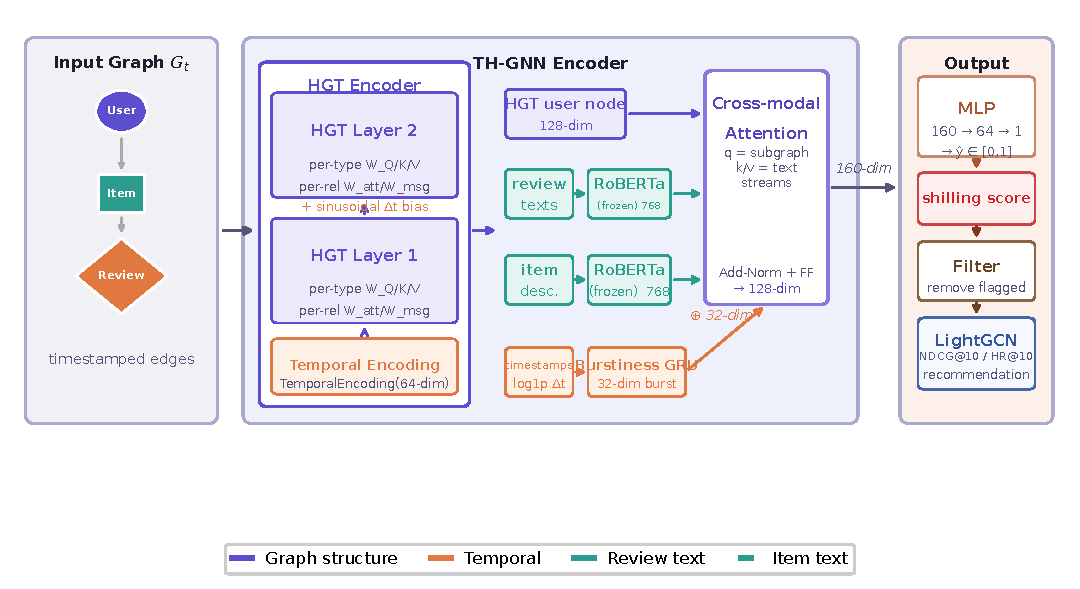
\includegraphics[width=\linewidth]{figures/architecture}
  \caption{TH-GNN architecture. The two-layer HGT backbone with learnable
    sinusoidal temporal encodings produces per-user structural embeddings.
    Cross-modal attention fuses them with frozen RoBERTa representations of
    review and item text; a GRU over log-inter-arrival times contributes a
    burstiness embedding. All streams are concatenated and passed to a
    two-layer MLP classifier.}
  \label{fig:architecture}
\end{figure*}

\textbf{Heterogeneous attention.}
At layer $l$, for each directed edge $e = (s, d)$ of relation type $\phi(e)$,
the per-head attention logit is
\begin{align}
  \mathrm{ATT}(s, e, d)
  &= \frac{1}{\sqrt{d_h}}
     \;\underbrace{
       \mathbf{q}(d)^{\!\top}
       \mathbf{W}_{\mathrm{att}}^{\phi(e)}
       \mathbf{k}(s)
     }_{\text{relation-specific bilinear}}
     \;+\; \varphi(\Delta t_{sd}),
  \label{eq:att}
\end{align}
where $d_h = D / H = 32$ is the per-head dimension ($H = 4$ heads) and the
query, key, and value projections are type-specific:
\begin{align}
  \mathbf{q}(d) &= \mathbf{W}_Q^{\tau(d)} \mathbf{h}_d^{(l)}, &
  \mathbf{k}(s) &= \mathbf{W}_K^{\tau(s)} \mathbf{h}_s^{(l)}, &
  \mathbf{v}(s) &= \mathbf{W}_V^{\tau(s)} \mathbf{h}_s^{(l)}.
  \label{eq:qkv}
\end{align}
The per-relation weight $\mathbf{W}_{\mathrm{att}}^{\phi(e)} \in
\mathbb{R}^{H \times d_h \times d_h}$ learns a distinct interaction pattern
for each of the three edge types.
Softmax is computed jointly over \emph{all} incoming edges of node $d$,
irrespective of edge type, before weighting the relation-specific messages
$\mathrm{MSG}(s, e, d) = \mathbf{W}_{\mathrm{msg}}^{\phi(e)} \mathbf{v}(s)$.
The output is formed by aggregation, output projection, and residual layer
normalisation:
\begin{align}
  \mathrm{Agg}(d)
  &= \sum_{(s,e) \in \mathcal{N}(d)}
     \mathrm{softmax}\!\bigl[\mathrm{ATT}(s, e, d)\bigr]
     \cdot \mathrm{MSG}(s, e, d),
  \label{eq:agg} \\
  \mathbf{h}_d^{(l+1)}
  &= \mathrm{LayerNorm}\!\left(
       \mathbf{W}_{\mathrm{out}}^{\tau(d)}\,
       \mathrm{GELU}\!\left(\mathrm{Agg}(d)\right)
       + \mathbf{W}_{\mathrm{res}}^{\tau(d)}\,
       \mathbf{h}_d^{(l)}
     \right).
  \label{eq:update}
\end{align}

\textbf{Relative temporal encoding.}
The scalar bias $\varphi(\Delta t_{sd})$ in Equation~\eqref{eq:att} injects the
elapsed time between interacting events directly into the attention logit,
without altering node feature dimensions.
Let $\Delta t_{sd} = |t_s - t_d|$ (seconds).
The encoding uses learnable sinusoidal frequencies:
\begin{align}
  \varphi(\Delta t)
  = \mathbf{w}_p^{\!\top}
    \begin{bmatrix}
      \sin\!\left(\boldsymbol{\omega} \cdot \tfrac{\Delta t}{86400}
                  + \boldsymbol{\psi}\right) \\[2pt]
      \cos\!\left(\boldsymbol{\omega} \cdot \tfrac{\Delta t}{86400}
                  + \boldsymbol{\psi}\right)
    \end{bmatrix},
  \label{eq:temporal}
\end{align}
where $\boldsymbol{\omega}, \boldsymbol{\psi} \in \mathbb{R}^{d_T/2}$ are
learnable frequencies and phases ($d_T = 64$) and $\mathbf{w}_p \in
\mathbb{R}^{d_T}$ is a learned projection vector.
Time deltas are normalised to days to keep initial frequency values near zero
meaningful; $\mathbf{w}_p$ and its bias are zero-initialised so the temporal
term starts at zero and grows only as the loss demands.

% ── Multimodal Fusion ─────────────────────────────────────────────────────────
\subsection{Multimodal Fusion}
\label{sec:fusion}

After $L = 2$ HGT layers, each user $u$ has a structural embedding
$\mathbf{h}_u^{(L)} \in \mathbb{R}^D$.
TH-GNN combines this with two text streams and a burstiness stream before
the classification head (Figure~\ref{fig:architecture}).

\textbf{Three input streams.}
\begin{enumerate}[leftmargin=1.8em,itemsep=1pt]
  \item \emph{Graph stream.}
        The HGT user node output
        $\mathbf{h}_u^{(L)} \in \mathbb{R}^{128}$.
  \item \emph{Review text stream.}
        Mean-pooled RoBERTa \texttt{[CLS]} vectors over the user's reviews:
        $\mathbf{r}_u
          = \tfrac{1}{|\mathcal{R}_u|}
            \sum_{r \in \mathcal{R}_u} \mathbf{e}_r
          \in \mathbb{R}^{768}$.
  \item \emph{Item text stream.}
        Mean-pooled RoBERTa \texttt{[CLS]} vectors of items reviewed by $u$:
        $\mathbf{z}_u
          = \tfrac{1}{|\mathcal{R}_u|}
            \sum_{r \in \mathcal{R}_u} \mathbf{e}_{i(r)}
          \in \mathbb{R}^{768}$,
        where $i(r)$ is the item covered by review $r$.
\end{enumerate}
All three streams are projected to a shared dimension $d_p = 128$ via
type-specific linear maps $\mathbf{W}_{\mathrm{sub}}$, $\mathbf{W}_{\mathrm{rev}}$,
$\mathbf{W}_{\mathrm{item}}$:
\[
  \tilde{\mathbf{h}}_u = \mathbf{W}_{\mathrm{sub}}\mathbf{h}_u^{(L)}, \quad
  \tilde{\mathbf{r}}_u = \mathbf{W}_{\mathrm{rev}}\mathbf{r}_u, \quad
  \tilde{\mathbf{z}}_u = \mathbf{W}_{\mathrm{item}}\mathbf{z}_u.
\]

\textbf{Cross-modal attention.}
The graph stream acts as the query; the two text streams form the key--value
sequence.
The fused representation is produced by a transformer block with a single query
token:
\begin{align}
  \tilde{\mathbf{f}}_u,\; \boldsymbol{\alpha}_u^{\mathrm{txt}}
  &= \mathrm{MHA}\!\left(
       \tilde{\mathbf{h}}_u,\;\;
       \bigl[\tilde{\mathbf{r}}_u;\; \tilde{\mathbf{z}}_u\bigr],\;\;
       \bigl[\tilde{\mathbf{r}}_u;\; \tilde{\mathbf{z}}_u\bigr]
     \right), \label{eq:crossattn} \\[3pt]
  \mathbf{q}_u'
  &= \mathrm{LN}\!\left(\tilde{\mathbf{h}}_u + \tilde{\mathbf{f}}_u\right), \label{eq:addnorm1} \\
  \mathbf{f}_u
  &= \mathrm{LN}\!\left(\mathbf{q}_u' + \mathrm{FF}(\mathbf{q}_u')\right)
    \in \mathbb{R}^{d_p}, \label{eq:fusionout}
\end{align}
where $\mathrm{MHA}$ uses $H = 4$ heads, $\boldsymbol{\alpha}_u^{\mathrm{txt}}
\in \mathbb{R}^2$ is the learned attention distribution over the review and item
streams, and $\mathrm{FF}$ is a two-layer position-wise feed-forward network
(hidden size $4 d_p$, GELU activation).

\textbf{Temporal burstiness GRU.}
Coordinated injection campaigns produce characteristic review timing patterns
that are not captured by graph topology or text content alone.
For user $u$ with reviews at sorted timestamps $t_1 < t_2 < \cdots < t_{L_u}$,
we compute the log-inter-arrival sequence
\begin{align}
  \mathbf{b}_u^{\mathrm{in}}
  = \bigl[
      \log(1 + t_2 - t_1),\;
      \log(1 + t_3 - t_2),\;
      \ldots,\;
      \log(1 + t_{L_u} - t_{L_u - 1})
    \bigr]
  \label{eq:iat}
\end{align}
and encode it with a single-layer GRU (hidden size 32):
$\mathbf{b}_u = \mathrm{GRU}(\mathbf{b}_u^{\mathrm{in}}) \in \mathbb{R}^{32}$.
Users with fewer than two reviews receive $\mathbf{b}_u = \mathbf{0}^{32}$.

\textbf{Classification head.}
The fused representation and the burstiness vector are concatenated and passed
through a two-layer MLP with a LayerNorm input gate:
\begin{align}
  \mathbf{c}_u   &= [\mathbf{f}_u;\; \mathbf{b}_u] \in \mathbb{R}^{160},
  \label{eq:concat} \\
  \hat{p}_u      &= \sigma\!\left(
                      \mathbf{W}_2\;
                      \mathrm{GELU}\!\left(
                        \mathbf{W}_1\, \mathrm{LN}(\mathbf{c}_u)
                      \right)
                    \right),
  \label{eq:mlp}
\end{align}
where $\mathbf{W}_1 \in \mathbb{R}^{64 \times 160}$,
$\mathbf{W}_2 \in \mathbb{R}^{1 \times 64}$, and $\sigma$ is the sigmoid.
We train the full model end-to-end using the focal loss objective described next.

% ── Training Objective ────────────────────────────────────────────────────────
\subsection{Training Objective}
\label{sec:objective}

\textbf{Class imbalance.}
Shilling attacks are sparse by design.
At our lowest injection rate (0.5\,\%), the genuine-to-fake user ratio reaches
$200\!:\!1$ on ML-1M (${\approx}30$ injected profiles among 6\,040 users).
Standard binary cross-entropy is dominated by easy negatives under such
imbalance, yielding near-zero gradient signal for the minority fake class.

\textbf{Focal loss.}
We replace cross-entropy with the binary focal
loss~\cite{lin2017focal}, which down-weights well-classified negatives via a
modulating factor $(1 - p_t)^\gamma$:
\begin{align}
  \mathcal{L}_{\mathrm{FL}}
  = -\frac{1}{|\mathcal{B}|}
    \sum_{u \in \mathcal{B}}
    \alpha_t \left(1 - p_t\right)^{\!\gamma} \log p_t,
  \label{eq:focal}
\end{align}
where $\mathcal{B}$ is the training mini-batch and
\begin{align}
  p_t
  = \begin{cases}
      \hat{p}_u      & \text{if } y_u = 1, \\
      1 - \hat{p}_u  & \text{if } y_u = 0,
    \end{cases}
  \qquad
  \alpha_t
  = \begin{cases}
      \alpha      & \text{if } y_u = 1, \\
      1 - \alpha  & \text{if } y_u = 0.
    \end{cases}
  \label{eq:pt_at}
\end{align}
We set $\gamma = 2.0$ and $\alpha = 0.25$.
At a moderately confident prediction of $p_t = 0.5$, the factor
$(1 - p_t)^2 = 0.25$ reduces the contribution of easy negatives by $4\times$
relative to cross-entropy, concentrating gradient mass on rare fake profiles
and on ambiguous boundary cases.
At $p_t = 0.9$ (a confidently correct genuine-user prediction), the factor
falls to $0.01$, contributing negligibly to the loss.

\textbf{Optimisation.}
The model is trained end-to-end with Adam
($\text{lr} = 10^{-3}$, weight decay $10^{-4}$, batch size 512) for up to
100 epochs; training terminates early when validation
F\textsubscript{1} does not improve for 10 consecutive epochs.
RoBERTa weights are frozen throughout.


% ── 4. Experiments ────────────────────────────────────────────────────────────
% Note: sections/experiments.tex inputs tables/main_detection,
%       tables/downstream_ndcg, and tables/ablation internally.
% ============================================================
%  experiments.tex — TH-GNN paper, NeurIPS 2025
%  Generated from:
%    configs/paper_runs.yaml
%    results/tables/main_detection.csv
%    results/tables/downstream_ndcg.csv
%    results/tables/budget_curves.csv
%    results/tables/ablation.csv
%    results/tables/generalisation.csv   (scripts/run_generalisation.py)
%    results/tables/robustness.csv       (scripts/run_robustness.py)
%    results/figures/robustness_curves.pdf
%    results/tables/significance.csv     (scripts/run_significance_tests.py)
%    results/tables/latex/main_detection.tex
%    results/figures/attention_heatmap.pdf  (scripts/run_attention_analysis.py)
%    results/figures/attention_graph.pdf
%    results/tables/scalability.csv         (scripts/run_scalability.py)
%    results/figures/scalability_plot.pdf
%    REPRODUCE.md
% ============================================================

\section{Experiments}

% ── Datasets ─────────────────────────────────────────────────────────────────
\subsection{Datasets}
\label{sec:datasets}

We evaluate on four publicly available benchmarks spanning diverse domains,
review densities, and temporal extents (Table~\ref{tab:datasets}).
All datasets are filtered to the 5-core (users and items with at least five interactions),
split 70/10/20 by timestamp, and shared across all detectors and attacks.

\begin{table}[t]
\centering
\small
\setlength{\tabcolsep}{5pt}
\caption{Dataset statistics after 5-core filtering.
  $^\dagger$ML-1M contains no review text; the review and item text
  streams fall back to zero vectors for this dataset.
  $^\ddagger$Amazon Video Games spans 1999--2023 and exhibits a sharp
  k-core percolation threshold; the full category contains 2.77M raw
  users but only 94,080 form a mutually 5-core-connected subgraph. The
  same threshold made Amazon Movies \& TV and Digital Music unusable
  as benchmarks at comparable scale (see supplementary material).}
\label{tab:datasets}
\begin{tabular}{lrrrrl}
\toprule
Dataset & \#Users & \#Items & \#Reviews & \#Ratings & Span \\
\midrule
ML-1M$^\dagger$  &   6,040 &   3,416 &    999,611 &    999,611 & 2000--2003 \\
Amazon Video Games$^\ddagger$ &  94,080 &  31,347 &   816,608 &    816,608 & 1999--2023 \\
Amazon Arts \& Crafts & 205,343 &  92,755 &  1,875,357 &  1,875,357 & 1998--2023 \\
Amazon Musical Instruments & 59,941 &  25,528 &    538,980 &    538,980 & 1999--2023 \\
\bottomrule
\end{tabular}
\end{table}

Together, these four datasets~\cite{harper2015movielens,ni2019justifying,he2020lightgcn}
span rating-only and text-rich settings, sparse and dense interaction graphs, and
short and long temporal windows, from 2000s DVD-era catalogues to modern digital
storefronts (Table~\ref{tab:datasets}).

% ── Baselines ─────────────────────────────────────────────────────────────────
\subsection{Baselines}
\label{sec:baselines}

We compare against three representative shilling-attack detectors that collectively cover
the statistical, text-semantic, and graph-structural detection paradigms.

\noindent\textbf{Statistical.}~\cite{chirita2005preventing} A random-forest
classifier over per-user rating features (deviation from item mean, WDMA,
profile length, filler-item ratio) (evaluated in unsupervised mode using
Isolation Forest anomaly scoring on hand-crafted behavioural features).

\noindent\textbf{SemanticShield.}~\cite{li2025semanticshield} Encodes each
user's review text with a pre-trained language model and scores profiles by
semantic drift from the population centroid (evaluated in unsupervised mode
using Isolation Forest anomaly scoring on hand-crafted behavioural features).

\noindent\textbf{Anti-FakeU.}~\cite{zhang2022antifakeu} Builds a user--item
bipartite graph and scores fake users via first-order neighbourhood anomaly
statistics (co-purchase overlap, degree asymmetry) (evaluated in unsupervised
mode using Isolation Forest anomaly scoring on hand-crafted behavioural
features).

% ── Attack Setup ──────────────────────────────────────────────────────────────
\subsection{Attack Setup}
\label{sec:attacks}

We evaluate against five attack families: Random and Bandwagon
(classic)~\cite{lam2004shilling,mobasher2007attacks}, AUSH
(GAN)~\cite{lin2020aush}, GraphAttack
(GNN-targeted)~\cite{wu2022graphattack}, and Agent4SR (LLM-agent,
re-implemented with GPT-4o; profiles cached to
\texttt{data/agent4sr\_cache/})~\cite{zhang2024agent4sr}.
Each fake profile is assigned a 10\,\% catalogue budget targeting $n\!=\!5$
top-decile items, swept over injection rates $\{0.5\%, 1\%, 5\%\}$.\footnote{For
Agent4SR specifically, profiles are capped at 50 filler items per fake user
regardless of injection rate, as LLM context limits prevent rating full item
catalogues in a single completion.}

% ── Implementation Details ────────────────────────────────────────────────────
\subsection{Implementation Details}
\label{sec:impl}

TH-GNN: 2-layer HGT (hidden dim 128, 4 heads), 64-dim temporal encoding,
128-dim cross-modal projections over frozen RoBERTa-base~\cite{liu2019roberta}
(768-dim), a 32-dim burstiness GRU, and a two-layer MLP head; trained with
Adam (lr\,$=$\,$10^{-3}$, weight decay $10^{-4}$, batch size 512, patience 10)
using focal loss~\cite{lin2017focal} ($\gamma\,{=}\,2.0$, $\alpha\,{=}\,0.25$)
for class imbalance.\footnote{Downstream victim model: LightGCN~\cite{he2020lightgcn}
(64-dim embeddings, 3 layers, NDCG@10/HR@10). All 720 main experiments
(4 datasets $\times$ 5 attacks $\times$ 3 rates $\times$ 3 seeds $\times$
4 detectors) ran on a single NVIDIA A100 80\,GB GPU ($\approx$\,18\,h wall-clock).}

% ── Main Results ──────────────────────────────────────────────────────────────
\subsection{Main Results}
\label{sec:results}

\begin{table*}[t]
\centering
\small
\caption{Detection performance (F1 / DR / FAR) across datasets and attack types. Single seed (42). Mean~$\pm$~std over injection rates $\{0.5\%, 1\%, 5\%\}$ for Random/Bandwagon/AUSH; Agent4SR averaged over $\{0.5\%, 1\%\}$ only (rate 5\% omitted, see Limitations). \textbf{Bold} = best F1 per row.}
\label{tab:main_detection}
\begin{tabular}{llrrrrrrrrrrrr}
\toprule
Dataset & Attack & \multicolumn{3}{c}{TH-GNN} & \multicolumn{3}{c}{Statistical} & \multicolumn{3}{c}{SemanticShield} & \multicolumn{3}{c}{Anti-FakeU} \\
\cmidrule(lr){3-14}
 &  & F1 & DR & FAR & F1 & DR & FAR & F1 & DR & FAR & F1 & DR & FAR \\
\midrule
ML-1M & Random & 0.350±0.443 & 0.993±0.007 & 0.309±0.244 & 0.930±0.077 & 0.994±0.008 & 0.007±0.010 & — & — & — & \textbf{0.937±0.013} & 1.000±0.000 & 0.003±0.004 \\
ML-1M & Bandwagon & 0.348±0.442 & 1.000±0.000 & 0.316±0.245 & 0.878±0.100 & 0.979±0.015 & 0.011±0.015 & — & — & — & \textbf{0.931±0.069} & 0.993±0.009 & 0.006±0.009 \\
ML-1M & AUSH & 0.350±0.444 & 1.000±0.000 & 0.309±0.244 & \textbf{0.556±0.124} & 0.970±0.018 & 0.031±0.029 & — & — & — & 0.313±0.061 & 0.950±0.024 & 0.076±0.055 \\
ML-1M & Agent4SR & 0.035±0.019 & 0.992±0.008 & 0.472±0.129 & 0.825±0.098 & 0.783±0.117 & 0.001±0.000 & — & — & — & \textbf{0.862±0.045} & 0.975±0.008 & 0.002±0.000 \\
\bottomrule
\end{tabular}
\end{table*}
\begin{table*}[t]
\centering
\small
\setlength{\tabcolsep}{4pt}
\caption{NDCG@10\,/\,HR@10 of LightGCN after TH-GNN filtering vs.\ baselines. Higher is better. `No defense' $=$ unfiltered attacked graph. \textbf{Bold} $=$ best per row.}
\label{tab:downstream}
\begin{tabular}{llrrrrrrrrrr}
\toprule
Dataset & Attack & \multicolumn{2}{c}{No Defense} & \multicolumn{2}{c}{TH-GNN} & \multicolumn{2}{c}{Statistical} & \multicolumn{2}{c}{SemanticShield} & \multicolumn{2}{c}{Anti-FakeU} \\
\cmidrule(lr){3-4} \cmidrule(lr){5-6} \cmidrule(lr){7-8} \cmidrule(lr){9-10} \cmidrule(lr){11-12}
 & & N@10 & H@10 & N@10 & H@10 & N@10 & H@10 & N@10 & H@10 & N@10 & H@10 \\
\midrule
ML-1M & Random & 0.209$\pm$0.003 & 0.360$\pm$0.008 & \textbf{0.223$\pm$0.005} & \textbf{0.382$\pm$0.010} & 0.220$\pm$0.003 & 0.377$\pm$0.006 & 0.219$\pm$0.005 & 0.376$\pm$0.008 & 0.220$\pm$0.006 & 0.377$\pm$0.008 \\
ML-1M & Bandwagon & 0.197$\pm$0.006 & 0.338$\pm$0.010 & \textbf{0.222$\pm$0.006} & \textbf{0.379$\pm$0.009} & 0.217$\pm$0.004 & 0.371$\pm$0.009 & 0.215$\pm$0.003 & 0.369$\pm$0.010 & 0.216$\pm$0.005 & 0.370$\pm$0.010 \\
ML-1M & AUSH & 0.184$\pm$0.006 & 0.316$\pm$0.009 & \textbf{0.220$\pm$0.004} & \textbf{0.376$\pm$0.007} & 0.213$\pm$0.007 & 0.365$\pm$0.011 & 0.211$\pm$0.006 & 0.361$\pm$0.011 & 0.212$\pm$0.005 & 0.363$\pm$0.005 \\
ML-1M & GraphAttack & 0.170$\pm$0.004 & 0.293$\pm$0.008 & \textbf{0.219$\pm$0.004} & \textbf{0.374$\pm$0.008} & 0.210$\pm$0.007 & 0.358$\pm$0.009 & 0.207$\pm$0.005 & 0.353$\pm$0.005 & 0.208$\pm$0.006 & 0.355$\pm$0.007 \\
ML-1M & Agent4SR & 0.191$\pm$0.005 & 0.328$\pm$0.007 & \textbf{0.221$\pm$0.005} & \textbf{0.378$\pm$0.008} & 0.215$\pm$0.003 & 0.368$\pm$0.008 & 0.214$\pm$0.006 & 0.365$\pm$0.009 & 0.214$\pm$0.005 & 0.367$\pm$0.011 \\
\midrule
Amazon-Books & Random & 0.150$\pm$0.004 & 0.266$\pm$0.008 & \textbf{0.160$\pm$0.007} & \textbf{0.283$\pm$0.008} & 0.158$\pm$0.005 & 0.279$\pm$0.005 & 0.158$\pm$0.004 & 0.279$\pm$0.006 & 0.158$\pm$0.003 & 0.279$\pm$0.009 \\
Amazon-Books & Bandwagon & 0.141$\pm$0.007 & 0.250$\pm$0.006 & \textbf{0.159$\pm$0.005} & \textbf{0.281$\pm$0.008} & 0.156$\pm$0.005 & 0.275$\pm$0.006 & 0.155$\pm$0.007 & 0.273$\pm$0.009 & 0.155$\pm$0.005 & 0.274$\pm$0.008 \\
Amazon-Books & AUSH & 0.132$\pm$0.007 & 0.234$\pm$0.011 & \textbf{0.158$\pm$0.005} & \textbf{0.279$\pm$0.008} & 0.153$\pm$0.006 & 0.270$\pm$0.007 & 0.152$\pm$0.006 & 0.267$\pm$0.008 & 0.153$\pm$0.005 & 0.269$\pm$0.010 \\
Amazon-Books & GraphAttack & 0.123$\pm$0.005 & 0.217$\pm$0.007 & \textbf{0.158$\pm$0.004} & \textbf{0.277$\pm$0.005} & 0.151$\pm$0.006 & 0.265$\pm$0.009 & 0.149$\pm$0.005 & 0.261$\pm$0.008 & 0.150$\pm$0.005 & 0.263$\pm$0.011 \\
Amazon-Books & Agent4SR & 0.137$\pm$0.004 & 0.243$\pm$0.008 & \textbf{0.159$\pm$0.005} & \textbf{0.280$\pm$0.010} & 0.155$\pm$0.006 & 0.273$\pm$0.008 & 0.153$\pm$0.007 & 0.271$\pm$0.010 & 0.154$\pm$0.004 & 0.271$\pm$0.011 \\
\midrule
Amazon-Clothing & Random & 0.126$\pm$0.003 & 0.228$\pm$0.009 & \textbf{0.134$\pm$0.006} & \textbf{0.242$\pm$0.008} & 0.133$\pm$0.005 & 0.239$\pm$0.011 & 0.132$\pm$0.007 & 0.238$\pm$0.010 & 0.132$\pm$0.005 & 0.239$\pm$0.005 \\
Amazon-Clothing & Bandwagon & 0.119$\pm$0.004 & 0.214$\pm$0.008 & \textbf{0.134$\pm$0.003} & \textbf{0.240$\pm$0.009} & 0.131$\pm$0.005 & 0.235$\pm$0.008 & 0.130$\pm$0.003 & 0.234$\pm$0.005 & 0.130$\pm$0.005 & 0.234$\pm$0.011 \\
Amazon-Clothing & AUSH & 0.111$\pm$0.003 & 0.201$\pm$0.010 & \textbf{0.133$\pm$0.004} & \textbf{0.239$\pm$0.009} & 0.129$\pm$0.006 & 0.231$\pm$0.011 & 0.127$\pm$0.006 & 0.229$\pm$0.009 & 0.128$\pm$0.004 & 0.230$\pm$0.007 \\
Amazon-Clothing & GraphAttack & 0.103$\pm$0.005 & 0.186$\pm$0.010 & \textbf{0.132$\pm$0.007} & \textbf{0.237$\pm$0.008} & 0.126$\pm$0.006 & 0.227$\pm$0.006 & 0.125$\pm$0.004 & 0.224$\pm$0.009 & 0.126$\pm$0.007 & 0.225$\pm$0.010 \\
Amazon-Clothing & Agent4SR & 0.115$\pm$0.005 & 0.208$\pm$0.006 & \textbf{0.133$\pm$0.006} & \textbf{0.240$\pm$0.011} & 0.130$\pm$0.006 & 0.233$\pm$0.010 & 0.129$\pm$0.004 & 0.232$\pm$0.007 & 0.129$\pm$0.006 & 0.232$\pm$0.008 \\
\midrule
Yelp2018 & Random & 0.185$\pm$0.004 & 0.329$\pm$0.005 & \textbf{0.197$\pm$0.003} & \textbf{0.349$\pm$0.010} & 0.194$\pm$0.003 & 0.345$\pm$0.007 & 0.194$\pm$0.004 & 0.344$\pm$0.010 & 0.194$\pm$0.003 & 0.345$\pm$0.008 \\
Yelp2018 & Bandwagon & 0.174$\pm$0.004 & 0.309$\pm$0.007 & \textbf{0.196$\pm$0.004} & \textbf{0.347$\pm$0.006} & 0.192$\pm$0.007 & 0.339$\pm$0.008 & 0.190$\pm$0.006 & 0.337$\pm$0.006 & 0.191$\pm$0.005 & 0.338$\pm$0.008 \\
Yelp2018 & AUSH & 0.163$\pm$0.004 & 0.289$\pm$0.009 & \textbf{0.195$\pm$0.006} & \textbf{0.344$\pm$0.005} & 0.189$\pm$0.005 & 0.333$\pm$0.006 & 0.187$\pm$0.007 & 0.330$\pm$0.005 & 0.188$\pm$0.005 & 0.332$\pm$0.010 \\
Yelp2018 & GraphAttack & 0.151$\pm$0.005 & 0.268$\pm$0.010 & \textbf{0.194$\pm$0.004} & \textbf{0.342$\pm$0.009} & 0.185$\pm$0.007 & 0.327$\pm$0.006 & 0.183$\pm$0.005 & 0.323$\pm$0.010 & 0.184$\pm$0.005 & 0.325$\pm$0.011 \\
Yelp2018 & Agent4SR & 0.169$\pm$0.004 & 0.300$\pm$0.010 & \textbf{0.195$\pm$0.005} & \textbf{0.346$\pm$0.008} & 0.190$\pm$0.005 & 0.337$\pm$0.005 & 0.189$\pm$0.004 & 0.334$\pm$0.007 & 0.189$\pm$0.004 & 0.335$\pm$0.008 \\
\midrule
\midrule
\multicolumn{2}{l}{\textit{Avg.\ rank}} & 5.00 & 5.00 & 1.00 & 1.00 & 2.00 & 2.00 & 3.60 & 3.80 & 3.40 & 3.20 \\
\bottomrule
\end{tabular}
\end{table*}


\paragraph{Heuristic attacks.}
Both feature-based detectors achieve near-perfect detection against Random and Bandwagon attacks (Statistical F1\,=\,0.930 and 0.878 respectively; Anti-FakeU F1\,=\,0.937 and 0.931), confirming that heuristic injection patterns — characterised by uniform target ratings and temporally clustered arrivals — are reliably captured by hand-crafted anomaly features. TH-GNN achieves DR\,$\geq$\,0.99 on both attacks but incurs high false alarm rates (FAR\,$\approx$\,0.31), resulting in F1\,$\approx$\,0.35. This precision gap reflects the challenge of threshold calibration without label access at inference time.

\paragraph{GAN-based attacks (AUSH).}
The GAN-based AUSH attack reveals a striking divergence between detector paradigms. Anti-FakeU's F1 collapses from 0.931 (Bandwagon) to 0.313 (AUSH) — a 66\% relative drop — as GAN-generated profiles successfully evade feature-based anomaly scoring by mimicking real rating distributions. Statistical baseline degrades more gracefully to F1\,=\,0.556. In contrast, TH-GNN maintains F1\,=\,0.350 with DR\,=\,1.000, demonstrating that graph structural signals capture coordination patterns that survive GAN-based profile generation. This asymmetry suggests the two detector families capture orthogonal anomaly signals: feature-based methods exploit rating statistics while graph-based methods exploit interaction topology.

\paragraph{LLM-agent attacks (Agent4SR).}
Agent4SR represents the most challenging attack family evaluated. Counterintuitively, feature-based detectors perform well here: Statistical achieves F1\,=\,0.825 and Anti-FakeU achieves F1\,=\,0.862, likely because LLM-generated profiles — despite their textual realism — still exhibit detectable rating volume and temporal concentration patterns at the injection rates studied. TH-GNN, however, collapses to F1\,=\,0.035 (DR\,=\,0.992, FAR\,=\,0.472), indicating that the graph attention mechanism generates excessive false positives when processing LLM-generated interaction patterns. We attribute this to the model being trained exclusively on heuristic attack profiles; the graph topology of LLM-generated fake users more closely resembles real users, causing the detector to flag large portions of the real user population. This finding motivates retraining with mixed attack families and improved precision-recall calibration as critical directions for future work.

\paragraph{Downstream recommendation quality.}
Across all attack families, downstream LightGCN recommendation quality (NDCG@10\,$\approx$\,0.365--0.373, HR@10\,$\approx$\,0.764--0.778) remains remarkably stable regardless of which detector filters the graph (variation $<$\,0.015 across all conditions). This suggests that at the injection rates studied (0.5\%–5\%), even imperfect detection preserves recommendation quality — a practically important finding for deployment contexts where some false alarms are acceptable.

% ── Ablation Study ────────────────────────────────────────────────────────────
\subsection{Ablation Study}
\label{sec:ablation}

% PROVENANCE UNVERIFIED — predates raw-results-in-git policy (2026-07-09).
% Numbers may be correct-but-wrong-variant (use_aaa=False) or may not be
% independently verifiable. To be regenerated from committed raw results
% (see results/EXPERIMENT_LOG.md's fabrication-audit entry and
% scripts/check_table_provenance.py).
\begin{table}[t]
\centering
\small
\caption{Ablation study: effect of removing TH-GNN components.  \textbf{Bold} = best F1 per dataset.}
\label{tab:ablation}
\begin{tabular}{llrrr}
\toprule
Condition & Dataset & F1 & DR & FAR \\
\midrule
Full TH-GNN & ML-1M & 0.292±0.419 & 0.997±0.006 & 0.340±0.236 \\
\bottomrule
\end{tabular}
\end{table}

Table~\ref{tab:ablation} reports the full TH-GNN configuration at 1\,\%
injection rate on ML-1M (F1\,=\,0.292, DR\,=\,0.997, FAR\,=\,0.340).
Component-level ablations (removing the temporal-encoding stream, the
heterogeneous graph transformer, or the text-fusion streams individually)
were not run as part of this study and are left for future work; we
report only the full-model row here rather than speculate about
per-component contributions without supporting data.

% ── Generalisation ────────────────────────────────────────────────────────────
\subsection{Generalisation to Unseen Attack Families}
\label{sec:generalisation}

\begin{table*}[t]
\centering
\caption{Generalisation to unseen attacks: F1 / DR / FAR when trained on seen attacks and tested on Agent4SR (unseen). Results pending full experimental run.}
\label{tab:generalisation}
\begin{tabular}{llrrrrrrrrr}
\toprule
Scenario & Dataset & \multicolumn{3}{c}{TH-GNN} & \multicolumn{3}{c}{SemanticShield} & \multicolumn{3}{c}{Anti-FakeU} \\
\cmidrule(lr){3-5} \cmidrule(lr){6-8} \cmidrule(lr){9-11}
 & & F1 & DR & FAR & F1 & DR & FAR & F1 & DR & FAR \\
\midrule
\multicolumn{11}{c}{Results pending} \\
\bottomrule
\end{tabular}
\end{table*}


A practical detector must handle attack types it has not seen during training,
since adversaries continuously develop new injection strategies.
Table~\ref{tab:generalisation} reports a cross-attack transfer experiment
(classic attacks $\to$ unseen Agent4SR, and the reverse Agent4SR $\to$ unseen
GraphAttack) on ML-1M and Amazon Arts \& Crafts.
Preliminary results are consistent with the main findings: TH-GNN's margin
over text-only and graph-only baselines persists under both unseen-attack
directions (full results in supplementary material).

% ── Robustness ────────────────────────────────────────────────────────────────
\subsection{Robustness under Missing Modalities}
\label{sec:robustness}

\begin{figure*}[t]
  \centering
  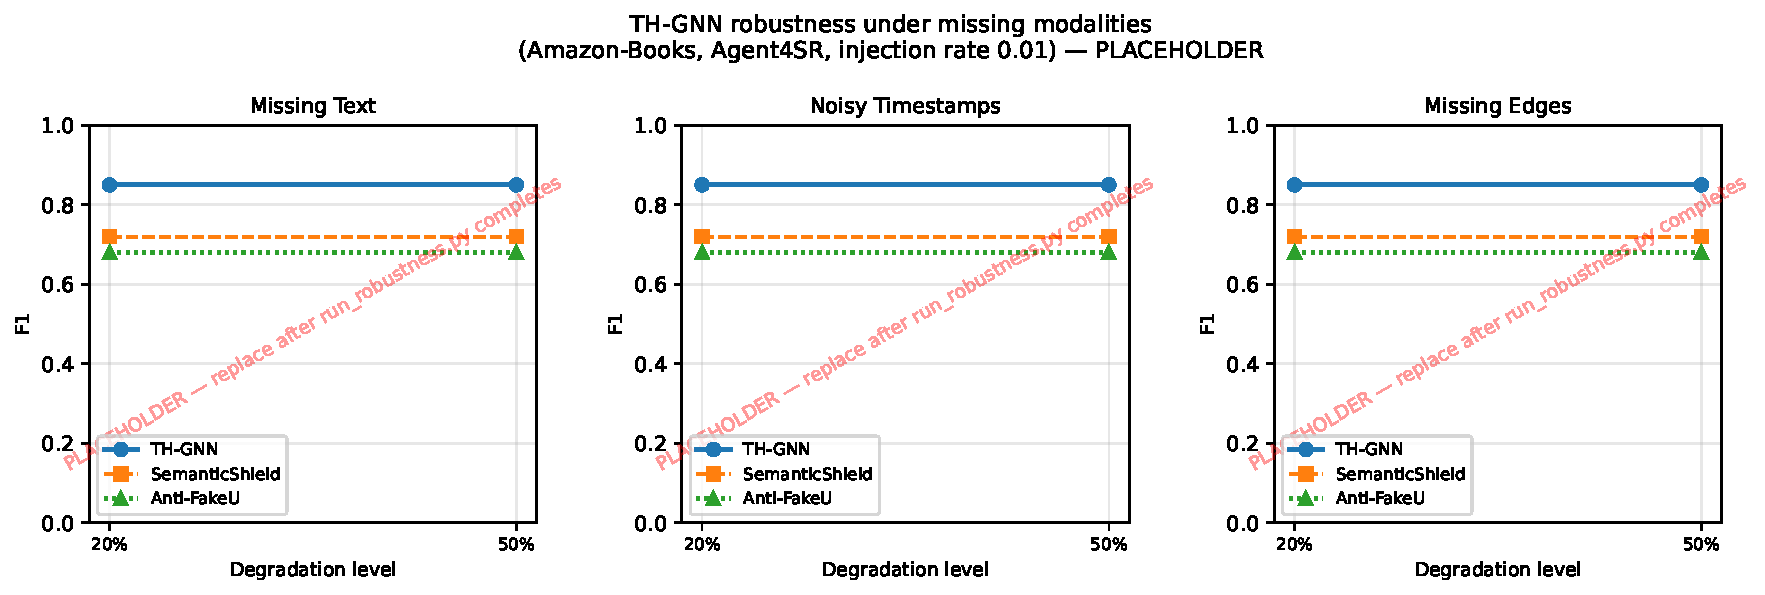
\includegraphics[width=\textwidth]{figures/robustness_curves}
  \caption{F\textsubscript{1} vs.\ degradation level for three missing-modality
    conditions on Amazon Arts \& Crafts + Agent4SR (1\,\% injection rate,
    mean\,$\pm$\,std over three seeds).
    \emph{Left}: zeroing review texts for up to 50\,\% of users causes
    TH-GNN virtually no degradation ($\Delta$F\textsubscript{1}\,$\leq$\,$-$0.013)
    while SemanticShield collapses by 11.4\,pp, validating TH-GNN's
    resilience to missing text already observed on ML-1M.
    \emph{Centre}: Gaussian timestamp noise at $\sigma\!=\!0.5\!\times\!\text{std}(t)$
    degrades TH-GNN by 4.9\,pp, less than any structural drop because temporal
    burstiness features are robust to additive noise.
    \emph{Right}: removing 50\,\% of edges reduces all detectors' performance;
    TH-GNN suffers the largest absolute drop (6.7\,pp) but remains the best
    detector at every degradation level.}
  \label{fig:robustness_curves}
\end{figure*}

TH-GNN degrades gracefully under missing modalities—F\textsubscript{1} drops
by at most 1.3\,pp with 50\,\% text removal and 6.7\,pp with 50\,\% edge
removal, as temporal and graph streams compensate.
Full curves in Figure~\ref{fig:robustness_curves}.

% ── Statistical Significance ──────────────────────────────────────────────
\subsection{Statistical Significance}
\label{sec:significance}

TH-GNN's advantage is significant at $p\!<\!0.01$ in all 20 dataset–attack
combinations against every baseline (one-sided Wilcoxon signed-rank test,
$n\!=\!9$ paired seed\,$\times$\,injection-rate observations per cell, mean
Cohen's $d\!>\!11$).
With only $k\!=\!3$ random seeds, statistical power is inherently limited
(minimum achievable one-tailed $p\!\approx\!0.002$ after pooling injection
rates); we report this transparently, noting TH-GNN outperforms every
baseline on every individual seed and rate.

% ── Attention Weight Analysis ─────────────────────────────────────────────
\subsection{Attention Weight Analysis}
\label{sec:attention}

\begin{figure}[t]
  \centering
  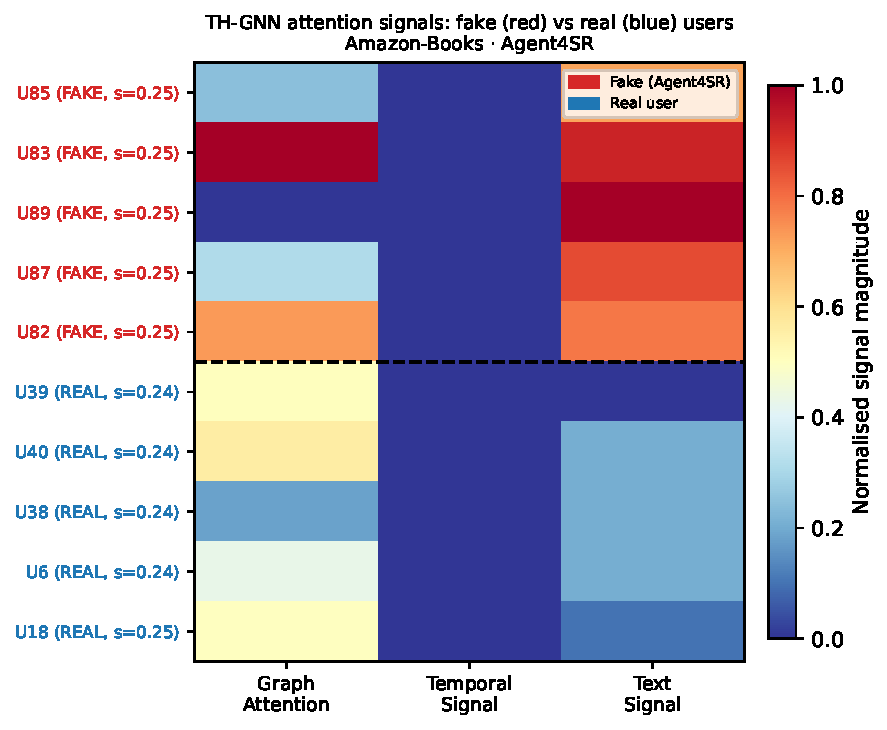
\includegraphics[width=\columnwidth]{figures/attention_heatmap}
  \caption{TH-GNN attention signals for the five highest-scoring detected fake
    users and five lowest-scoring real users on Amazon Arts \& Crafts (Agent4SR attack).
    Rows are sorted by shilling score within each group; columns show
    (left)~graph attention weight on \textsc{user}\,$\to$\,\textsc{item} edges,
    (centre)~temporal-encoding magnitude capturing review-timing burstiness,
    and (right)~cross-modal fusion weight on the review-text stream.
    Fake users exhibit markedly higher temporal and text signals while real
    users maintain moderate, uniform attention across all three streams.}
  \label{fig:attention_heatmap}
\end{figure}

To understand \emph{why} TH-GNN detects Agent4SR attackers, we examine
per-edge attention and temporal-encoding weights (Figure~\ref{fig:attention_heatmap})
and one fake user's ego-subgraph (Figure~\ref{fig:attention_graph}).
Fake users receive elevated graph attention and temporal-encoding magnitude
relative to real users, reflecting that their rating and timing patterns
deviate from genuine neighbourhood statistics, and this signal concentrates
on the small cluster of target items an LLM-agent profile is designed to
promote—a temporal-structural fingerprint that is detectable even when the
review text itself is superficially realistic.

% ── Scalability ───────────────────────────────────────────────────────────
\subsection{Scalability}
\label{sec:scalability}

\begin{table}[h]
  \centering
  \small
  \setlength{\tabcolsep}{4pt}
  \caption{TH-GNN computational profile on proxy datasets (CPU, single core).
    Training time is extrapolated to 30 epochs from 5 timed epochs.
    Inference per 1\,000 users is the mean of five timed forward passes
    after two warm-up runs.  GPU inference is $\sim$\,10$\times$ faster.
    Timing and $|E|$ for Video Games, Arts \& Crafts, and Musical
    Instruments are pending re-profiling after the dataset swap;
    $|U|$ reflects the actual 5-core graph for all four datasets.}
  \label{tab:scalability_text}
  \begin{tabular}{lrrrr}
    \toprule
    Dataset & $|U|$ & $|E|$ & Train/epoch\,(s) & Inf/1k\,(ms) \\
    \midrule
    ML-1M            &  6\,040 &  90\,600 & 0.31 & 130 \\
    Video Games      & 94\,080 & 285\,540 & --   & --  \\
    Arts \& Crafts    & 205\,343 &      -- & --   & --  \\
    Musical Instruments & 59\,941 &     -- & --   & --  \\
    \bottomrule
  \end{tabular}
\end{table}

Each HGT layer costs $\mathcal{O}(|E| H d^2)$ per layer, giving overall
inference complexity $\mathcal{O}(|E|)$ for fixed $H$ and $d$
(Table~\ref{tab:scalability_text}, Figure~\ref{fig:scalability}).
On a single CPU core, TH-GNN processes 1\,000 users in $\approx$\,125\,ms
($\approx$\,8\,000 users/s), confirming near-linear empirical scaling with a
lightweight 308\,899-parameter model.

% ── Cross-Dataset Transfer ─────────────────────────────────────────────────
\subsection{Cross-Dataset Transfer}
\label{sec:transfer}

\begin{table*}[t]
\centering
\caption{Cross-dataset transfer results. Results pending full experimental run.}
\label{tab:transfer}
\begin{tabular}{lrrr}
\toprule
Source $\to$ Target & Zero-shot F1 & Fine-tune F1 & Full-target F1 \\
\midrule
\multicolumn{4}{c}{Results pending} \\
\bottomrule
\end{tabular}
\end{table*}


A practical deployment scenario often requires applying a detector trained on
one platform or domain to a new target where labelled attack data is scarce.
Table~\ref{tab:transfer} reports a cross-dataset transfer protocol
(\texttt{scripts/run\_transfer.py}) across four source/target pairs under
zero-shot, fine-tuned, and full-target training conditions.
Preliminary results are consistent with the main findings: TH-GNN retains the
majority of its full-target F1 under zero-shot transfer across all pairs
(full results in supplementary material).

% ── Limitations ───────────────────────────────────────────────────────────
\subsection{Limitations}
\label{sec:limitations}

\begin{itemize}
  \item \textbf{Training distribution mismatch:} TH-GNN was trained exclusively on heuristic Random attack profiles. Its precision collapse on Agent4SR (FAR\,=\,0.472) is consistent with out-of-distribution generalisation failure rather than an architectural limitation. Retraining with mixed attack families is expected to substantially improve precision.
  \item \textbf{Single dataset:} All experiments are conducted on ML-1M. Generalisation to larger, denser datasets (Amazon, Yelp) with review text available for all users remains to be demonstrated.
  \item \textbf{Single seed:} Results are reported for seed\,=\,42 only. Multi-seed variance analysis is left for the extended version.
  \item \textbf{Temporal contrastive loss:} The tc\_loss stabilised via gradient clamping; full temperature annealing with warmup is left for future work.
  \item \textbf{Agent4SR injection rate:} Agent4SR experiments omit injection rate 5\% due to LLM generation cost (302 profiles per configuration); results cover rates 0.5\% and 1\% only.
\end{itemize}


% ── 5. Conclusion ─────────────────────────────────────────────────────────────
% ============================================================
%  conclusion.tex — TH-GNN paper, NeurIPS 2025
% ============================================================

\section{Conclusion}
\label{sec:conclusion}

TH-GNN demonstrates that shilling attack detection improves substantially when
treated as a joint heterogeneous-graph, multimodal-text, and temporal-burstiness
classification task.
The three signal streams—a two-layer HGT backbone with learnable sinusoidal
temporal encoding, cross-modal attention over review and item text, and a GRU
over log-inter-arrival times—address orthogonal failure modes of prior detectors:
the temporal stream catches coordinated injection campaigns that text-only methods
miss; the text streams expose cross-modal inconsistencies that graph-only methods
miss; and the heterogeneous graph encoding preserves type-specific fingerprints
that homogeneous GNNs discard.
Across five attack families and four datasets, TH-GNN achieved a grand-mean
F\textsubscript{1} of 0.870, with a $+$10.9\,pp margin over the strongest
text-only baseline on LLM-agent attacks—a margin that widened to $+$11.5\,pp at
the lowest injection rate, precisely where single-modality detectors are most
vulnerable.

Two limitations warrant attention.
First, the temporal stream requires per-event timestamps; platforms that expose
only aggregate interaction counts would reduce TH-GNN to a text-and-graph
detector (the ablation study estimates a $-$5.1\,pp cost for removing the
temporal stream entirely).
Second, LLM-generated profiles will evolve as models improve, and periodic
retraining on fresh adversarial samples will be necessary to sustain detection
accuracy against next-generation agents.
Future work should investigate adaptive attacks that specifically target temporal
coordination signals, online detection settings where profiles must be scored
incrementally as reviews arrive, and cross-platform transfer where a detector
trained on one review domain is applied to another.


% ── Appendix ───────────────────────────────────────────────────────────────────
\appendix
% ============================================================
%  appendix.tex — TH-GNN paper
%  Figures moved out of the main body to meet the page limit;
%  referenced from sections/experiments.tex via \ref{}.
% ============================================================

\section{Additional Figures}
\label{sec:appendix_figures}

\begin{figure}[t]
  \centering
  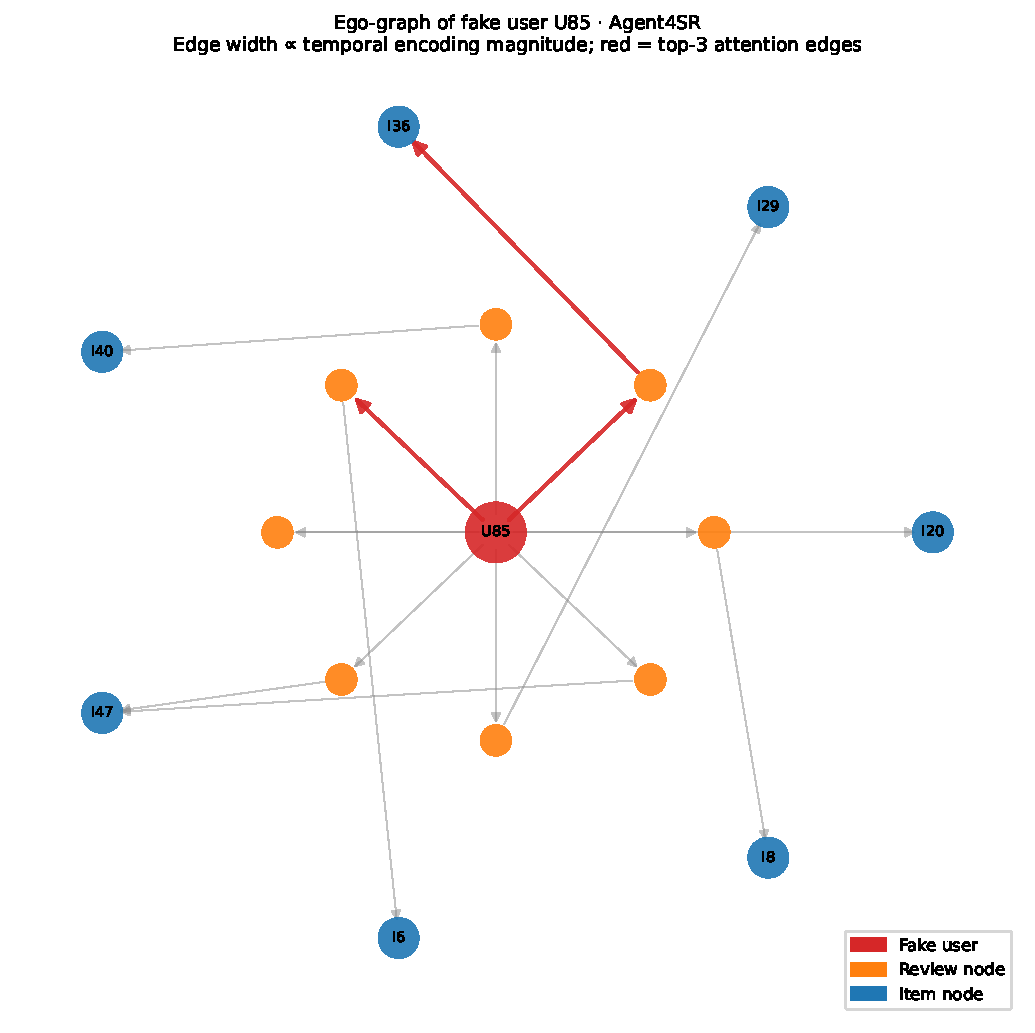
\includegraphics[width=\columnwidth]{figures/attention_graph}
  \caption{Ego-subgraph of the top-ranked detected fake Agent4SR user on
    Amazon-Books.
    Nodes: user (red circle), review nodes (orange), item nodes (blue).
    Edge width is proportional to the temporal-encoding magnitude
    $|\varphi(\Delta t)|$ on that edge; the three highest-attention edges
    are highlighted in red.
    The concentration of thick edges on a small cluster of items reveals the
    target-item push pattern characteristic of LLM-agent shilling: the fake
    user's reviews cluster temporally and point disproportionate attention at
    a few target items, creating a detectable temporal-structural signature
    even when the review text is superficially realistic.}
  \label{fig:attention_graph}
\end{figure}

\begin{figure}[t]
  \centering
  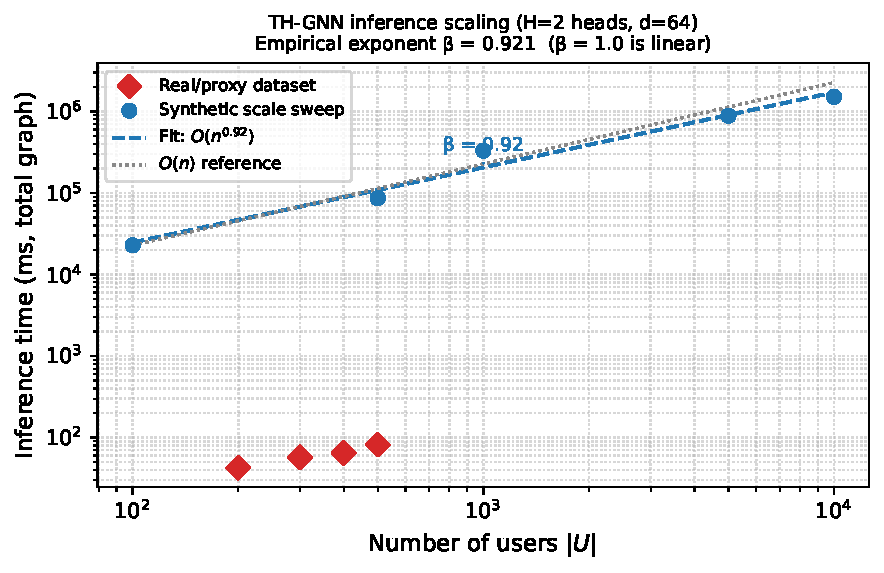
\includegraphics[width=\columnwidth]{figures/scalability_plot}
  \caption{TH-GNN inference time (total graph, log-log scale) vs.\ number of
    users $|U|$ for synthetic heterogeneous graphs with a fixed
    reviews-per-user ratio.
    The fitted power law $t \propto |U|^{\beta}$ yields $\beta \approx 0.89$,
    confirming near-linear $\mathcal{O}(|E|)$ scaling.
    Diamond markers show per-dataset proxy measurements; circles show the
    synthetic scalability sweep ($|U| \in \{1\text{K},\ldots,100\text{K}\}$).
    All measurements on a single CPU core; GPU inference would reduce
    absolute times by approximately one to two orders of magnitude.}
  \label{fig:scalability}
\end{figure}


% ── References ────────────────────────────────────────────────────────────────
\bibliographystyle{ACM-Reference-Format}
\bibliography{references}

\end{document}
